\documentclass[a4paper]{article}
\usepackage{a4wide,amssymb,epsfig,latexsym,array,hhline,fancyhdr}
\usepackage[normalem]{ulem}
\usepackage[makeroom]{cancel}
\usepackage{amsmath}
\usepackage{amsthm}
\usepackage{float}
\usepackage{multicol,longtable,amscd}
\usepackage{diagbox}%Make diagonal lines in tables
\usepackage{booktabs}
\usepackage{alltt}
\usepackage[framemethod=tikz]{mdframed}% For highlighting paragraph backgrounds
\usepackage{caption,subcaption}
\usepackage{lastpage}
\usepackage[lined,boxed,commentsnumbered]{algorithm2e}
\usepackage{enumerate}
\usepackage{color}
\usepackage{graphicx}							% Standard graphics package
% Code space
\usepackage{mdframed}
\usepackage{xcolor}
\usepackage{minted} % needs --shell-escape flag

\usepackage{array}
\usepackage{tabularx, caption}
\usepackage{multirow}
\usepackage{multicol}
\usepackage{rotating}
\usepackage{graphics}
\usepackage{geometry}
\usepackage{setspace}
\usepackage{epsfig}
\usepackage{tikz}
\usepackage{enumitem}
\usetikzlibrary{arrows,snakes,backgrounds}
\usepackage[unicode]{hyperref}
\hypersetup{urlcolor=blue,linkcolor=black,citecolor=black,colorlinks=true} 
\setlength{\parindent}{0pt}
\usepackage[normalem]{ulem}
\def\thesislayout{	% A4: 210 × 297
	\geometry{
		a4paper,
		total={160mm,240mm},  % fix over page
		left=30mm,
		top=30mm,
	}
}
\thesislayout

%\usepackage{fancyhdr}
\setlength{\headheight}{40pt}
\pagestyle{fancy}
\fancyhead{} % clear all header fields
\fancyhead[L]{
 \begin{tabular}{rl}
    \begin{picture}(25,15)(0,0)
    \put(0,-8){
\includegraphics[width=8mm, height=8mm]{Images/Logo BK.png}}
    %\put(0,-8){\epsfig{width=10mm,figure=hcmut.eps}}
   \end{picture}&
	%\includegraphics[width=8mm, height=8mm]{hcmut.png} & %
	\begin{tabular}{l}
		\textbf{\bf \ttfamily Ho Chi Minh City University of Technology}\\
	\end{tabular} 	
 \end{tabular}
}
\fancyhead[R]{
	\begin{tabular}{l}
		\tiny \bf \\
		\tiny \bf 
	\end{tabular}  }
\fancyfoot{} % clear all footer fields
\fancyfoot[L]{\scriptsize \ttfamily Probability and Statistics Project - 212 Semester}
\fancyfoot[R]{\scriptsize \ttfamily Page {\thepage}/\pageref{LastPage}}
\renewcommand{\headrulewidth}{0.3pt}
\renewcommand{\footrulewidth}{0.3pt}


\everymath{\color{blue}}%make in-line maths symbols blue to read/check easily
\sloppy
\captionsetup[figure]{labelfont={small,bf},textfont={small,it},}
%space remove between caption, figure, and text
\captionsetup[table]{labelfont={small,bf},textfont={small,it},}
\setlength{\floatsep}{5pt plus 2pt minus 2pt}
\setlength{\textfloatsep}{5pt plus 2pt minus 2pt}
\setlength{\intextsep}{10pt plus 2pt minus 2pt}

\thesislayout
\begin{document}
\begin{titlepage}
\begin{center}
VIETNAM NATIONAL UNIVERSITY \\
HO CHI MINH CITY UNIVERSITY OF TECHNOLOGY \\
OFFICE FOR INTERNATIONAL STUDY PROGRAMS 
\end{center}

\vspace{1cm}

\begin{figure}[h!]
\begin{center}

\includegraphics[width=0.6\linewidth]{Images/Logo BK.png}
\end{center}
\end{figure}

\vspace{1cm}


\begin{center}
\begin{tabular}{c}
\multicolumn{1}{l}{\textbf{{\Large PROBABILITY AND STATISTICS (MT2013)}}}\\
~~\\
\hline
\\

\textbf{\large PROJECT REPORT} \\
\textbf{\large Class: CC11   ------   Group: 2}\\

\hline
\end{tabular}
\end{center}

\vspace{1.5cm}


%%%%%%%%%%%%%%%%%%%%%%%%%%%%%%%%%%%%%%%%%%%%%%%%%%%%%%%%%%%%%%%%%%%%%%%%%%%%
%%%%%%%%%%%%%%%%%%%%%%%%%%%%%%%%%%%%%%%%%%%%%%%%%%%%%%%%%%%%%%%%%%%%%%%%%%%%

\begin{table}[h]
\begin{tabular}{rrl}
\hspace{5 cm} & Under the guidance of: & DR. PHAN THI HUONG\\

& Accomplished by: & \href{mailto:huy.le0107@hcmut.edu.vn}{LE GIA HUY} -- 1952717 \\
&                  & \href{mailto:dang.pham1310@hcmut.edu.vn}{PHAM THIEN DANG} -- 1952653 \\
&                  & \href{mailto:son.hoangthe@hcmut.edu.vn}{HOANG THE SON} -- 2053399 \\
&                  & \href{mailto:hung.nguyenskr2509@hcmut.edu.vn}{NGUYEN NGOC HUNG} -- 2053075 \\
&                  & \href{mailto:thien.tran31@hcmut.edu.vn}{TRAN QUANG THIEN} -- 2053455 \\
\end{tabular}

\end{table}
\vspace{1.5cm}
\begin{center}
{\footnotesize Ho Chi Minh City, March 2022}
\end{center}
\end{titlepage}

%%%%%%%%%%%%%%%%%%%%%%%%%%%%%%%%%%%%%%%%%%%%%%%%%%%%%%%%%%%%%%%%%%%%%%%%%%%%
%%%%%%%%%%%%%%%%%%%%%%%%%%%%%%%%%%%%%%%%%%%%%%%%%%%%%%%%%%%%%%%%%%%%%%%%%%%%

\tableofcontents
\newpage
\noindent
\section*{\textcolor{blue}{PROLOUGE}}
\addcontentsline{toc}{section}{\textcolor{blue}{PROLOUGE}}
\noindent
It is the moment for the project. This time, the project is mainly dealt with \textit{multiple linear regression} problems as well as a number of \textit{descriptive statistics} techniques. As we were stated in the previous report, all the outputs of R’s computation, rather than captured in the RStudio environment, are showed directly from the command line console; which somewhat eases up our inspection thanks to high contrast and standout texts. Moreover, instead showing the whole R codes at the end of each question, this time the code snippets will be show  along with the explanation texts during the demonstration. The structure of the report will also be more specific with a bunch of subsections for each activity. You will find the question, the procedure was carried out to attain the conclusion, and a brief summary for each problem along the way. Again, the assignment table is located at the last section of the document, where you will find the detailed descriptions of the tasks of each member in this project and their according percentage workload. \\ \newline
Now that it is enough for setting up the context, more will be explained 
when you walk through the document. To get an accomplished report, the team would like to give our instructor (Dr. Phan Thi Huong) a big appreciation for her great effort in helping in all the concepts of this course.


%%%%%%%%%%%%%%%%%%%%%%%%%%%%%%%%%%%%%%%%%%%%%%%%%%%%%%%%%%%%%%%%%%%%%%%%%%%%
%%%%%%%%%%%%%%%%%%%%%%%%%%%%%%%%%%%%%%%%%%%%%%%%%%%%%%%%%%%%%%%%%%%%%%%%%%%%

\vspace{3cm}
\section*{\textcolor{blue}{Member list \& Workload}}
\addcontentsline{toc}{section}{\textcolor{blue}{Member list \& Workload}}
\begin{table}[H]
\begin{tabular}{|l|l|l|l|l|}
\hline
\textbf{No.} 
& \textbf{\begin{tabular}{>{\centering\arraybackslash}m{3cm}} Fullname \end{tabular}}    
& \textbf{Student ID} 
& \textbf{\begin{tabular}{>{\centering\arraybackslash}m{5.5cm}} Problems \end{tabular}}    
& \textbf{Work Percentage}                                                                  
                                      \\ \hline
\textbf{\begin{tabular}{>{\centering\arraybackslash}m{0.3cm}} 1 \end{tabular}}   
& Le Gia Huy   
& \begin{tabular}{>{\centering\arraybackslash}m{1.5cm}} 1952717 \end{tabular}  
& \begin{tabular}[c]{@{}l@{}}- Accomplished Activity 1 \end{tabular} 
& \begin{tabular}{>{\centering\arraybackslash}m{2.5cm}} 100\% \end{tabular}                                           \\ \hline
\textbf{\begin{tabular}{>{\centering\arraybackslash}m{0.3cm}} 2 \end{tabular}}   
& Pham Thien Dang
& \begin{tabular}{>{\centering\arraybackslash}m{1.5cm}} 1952653 \end{tabular}  
& \begin{tabular}[c]{@{}l@{}}- Accomplished the Latex report \end{tabular} 
& \begin{tabular}{>{\centering\arraybackslash}m{2.5cm}} 100\% \end{tabular}   
                                      \\ \hline
\textbf{\begin{tabular}{>{\centering\arraybackslash}m{0.3cm}} 3 \end{tabular}}   
& Hoang The Son         
& \begin{tabular}{>{\centering\arraybackslash}m{1.5cm}} 2053399 \end{tabular}  
& \begin{tabular}[c]{@{}l@{}}- Accomplished Activity 2 \end{tabular} 
& \begin{tabular}{>{\centering\arraybackslash}m{2.5cm}} 100\% \end{tabular}   
                                      \\ \hline
\textbf{\begin{tabular}{>{\centering\arraybackslash}m{0.3cm}} 4 \end{tabular}}   
& Nguyen Ngoc Hung       
& \begin{tabular}{>{\centering\arraybackslash}m{1.5cm}} 2053075 \end{tabular} 
& \begin{tabular}[c]{@{}l@{}}- Accomplished Activity 2 \end{tabular} 
& \begin{tabular}{>{\centering\arraybackslash}m{2.5cm}} 100\% \end{tabular}   
                                      \\ \hline
\textbf{\begin{tabular}{>{\centering\arraybackslash}m{0.3cm}} 5 \end{tabular}}   
& Tran Quang Thien     
& \begin{tabular}{>{\centering\arraybackslash}m{1.5cm}} 2053455 \end{tabular} 
& \begin{tabular}[c]{@{}l@{}}- Accomplished Activity 2 \end{tabular} 
& \begin{tabular}{>{\centering\arraybackslash}m{2.5cm}} 100\% \end{tabular}   
                                      \\ \hline
\end{tabular}
\label{tab:memberlist}
\end{table}

%%%%%%%%%%%%%%%%%%%%%%%%%%%%%%%%%%%%%%%%%%%%%%%%%%%%%%%%%%%%%%%%%%%%%%%%%%%%
%%%%%%%%%%%%%%%%%%%%%%%%%%%%%%%%%%%%%%%%%%%%%%%%%%%%%%%%%%%%%%%%%%%%%%%%%%%%

\newpage
\section{\textcolor{blue}{Activity 1}}
\noindent
\subsection{Problem}
\vspace{0.4cm}
This data approach student achievement in secondary education of two Portuguese schools. The data attributes include student grades, demographic, social and school related features and it was collected by using school reports and questionnaires. \\ \\
Attribute Information:
\begin{itemize}
    \item[$\blacksquare$] \textit{sex} - student’s sex (binary: $F$ - \textbf{female} or $M$ - \textbf{male})
    \item[$\blacksquare$] \textit{age} - student’s age (numeric: from \textbf{15} to \textbf{22})
    \item[$\blacksquare$] \textit{studytime} - weekly study time ($1$: \textless{} 2 hours, $2$: 2 to 5 hours, $3$: 5 to 10 hours, or $4$: \textgreater{} 10 hours)
    \item[$\blacksquare$] \textit{failures} - number of past class failures (numeric: \textit{n} if $1 \leq n < 3$, else $4$). 
    \item[$\blacksquare$] \textit{higher} - wants to take higher education (binary: \textbf{yes} or \textbf{no})
    \item[$\blacksquare$] \textit{absences} - number of school absences (numeric: from \textbf{0} to \textbf{93}) 
    \item[$\blacksquare$] These grades are related with the course subject, Math or Portuguese:
    \begin{itemize}
        \item[\textbullet] \textit{G1} - first period grade (numeric: from \textbf{0} to \textbf{20})
        \item[\textbullet] \textit{G2} - second period grade (numeric: from \textbf{0} to \textbf{20})
        \item[\textbullet] \textit{G3} - final grade (numeric: from \textbf{0} to \textbf{20}, output target) 
    \end{itemize}
\end{itemize} 
Steps:
\begin{enumerate}
    \item Import data: \textbf{grade.csv} 
    \item Data cleaning: \textbf{NA} (Not available)
    \item Data visualization 
    \begin{enumerate}
        \item[(a)] Transformation (if it is necessary)
        \item[(b)] Descriptive statistics for each of the variables
        \item[(c)] Graphs: hist, boxplot, pairs
    \end{enumerate}
    \item Fitting linear regression models: We want to explore what factors may affect the final grade.
    \item Predictions.
\end{enumerate}

%%%%%%%%%%%%%%%%%%%%%%%%%%%%%%%%%%%%%%%%%%%%%%%%%%%%%%%%%%%%%%%%%%%%%%%%%%%%%

\vspace{0.5cm}
\subsection{Solution}
\vspace{0.4cm}
\subsubsection{Import data}
\vspace{0.4cm}
At first, installing the libraries for commands and functions is needed to solve the problem in a clear way.
\begin{enumerate}
    \item Installing the packages: 
    \begin{mdframed}[leftline=false,rightline=false,backgroundcolor=magenta!10,nobreak=true]
        \begin{minted}[linenos,breaklines,breaksymbolleft=,obeytabs=true,tabsize=2]{R}
install.packages("dplyr")
install.packages("GGally")
install.packages("broom")
install.packages("ggpubr")
        \end{minted}
    \end{mdframed}
    \item Calling the libraries:
    \begin{mdframed}[leftline=false,rightline=false,backgroundcolor=magenta!10,nobreak=true]
        \begin{minted}[linenos,breaklines,breaksymbolleft=,obeytabs=true,tabsize=2]{R}
library(ggplot2)
library(devtools)
library(GGally)
library(dplyr)
library(broom)
        \end{minted}
    \end{mdframed}
\end{enumerate}
After building a group of libraries, inputting the dataset and organizing the variables or factors from the dataset in columns are the following steps.
\begin{mdframed}[leftline=false,rightline=false,backgroundcolor=magenta!10,nobreak=true]
    \begin{minted}[linenos,breaklines,breaksymbolleft=,obeytabs=true,tabsize=2]{R}
#https://drive.google.com/file/d/1Nie3wexDWgIury6Tl3LSuHAvV15joJWz/view?usp=sharing
system("gdown --id 1xBHBU-hB6K4xQv4UTFEzcvjyQKqWWjpZ")
gradeData <- read.table("grade.csv", header = TRUE, sep = ",")
View(gradeData)
    \end{minted}
\end{mdframed}
And here for the result via using the \textit{dim(gradeData)} command:
\begin{figure}[H]
    \centering
    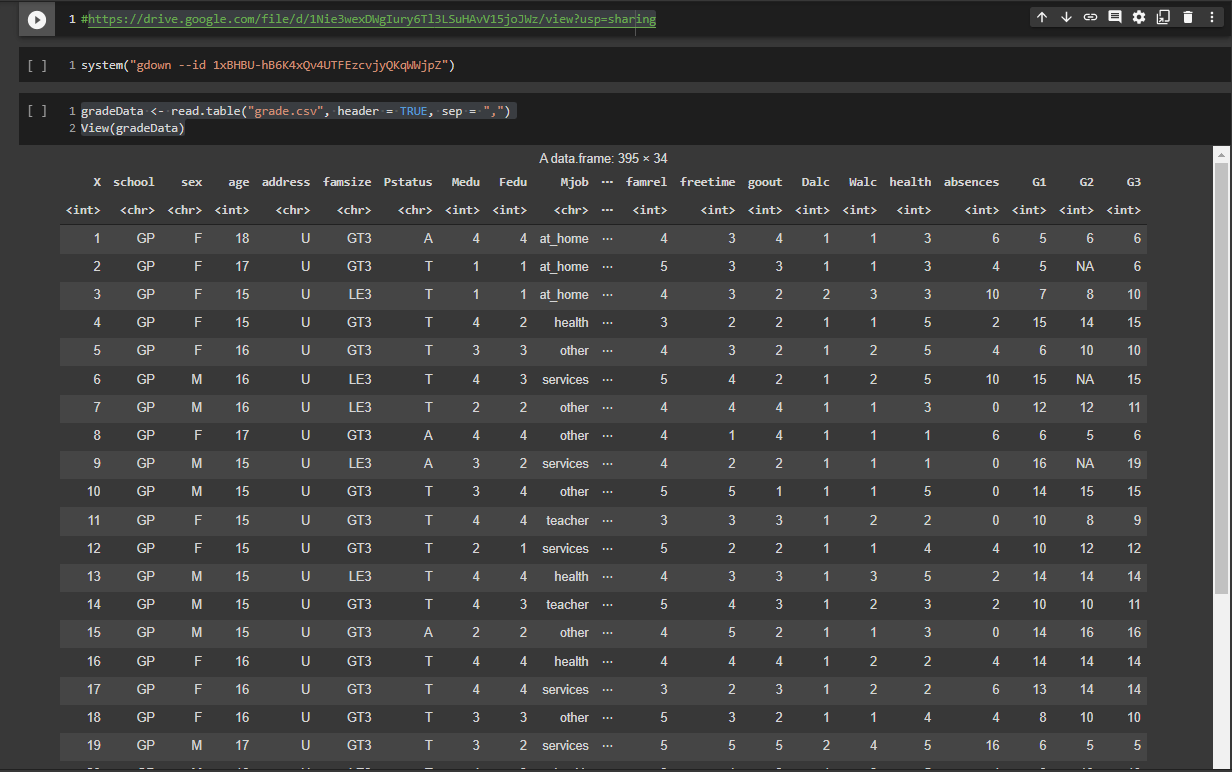
\includegraphics[scale = 0.7]{Images/1.PNG}
    \caption{There are 395 students whose information collected and 34 attributes corresponding to each student}
    \label{fig:dataset}
\end{figure}

%%%%%%%%%%%%%%%%%%%%%%%%%%%%%%%%%%%%%%%%%%%%%%%%%%%%%%%%%%%%%%%%%%%%%%%%%%%%

\subsubsection{Data cleaning: NA} 
\vspace{0.4cm}
Locating the null value in any factors and replacing them is the significant stage in data cleaning. In order to complete this step, by using the \textit{summary(gradeData)} command.
\begin{figure}[H]
    \centering
    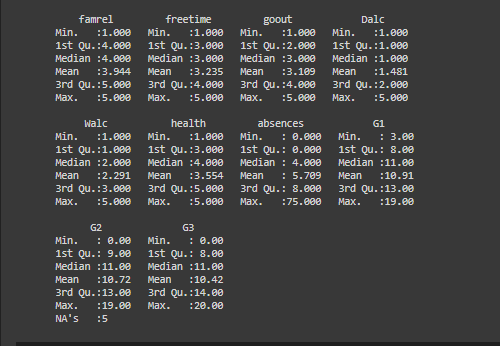
\includegraphics[scale = 1]{Images/2.PNG}
    \caption{There are 5 NA values in G2 column}
    \label{fig:summary}
\end{figure}
So the next step is the change in those values into the median calculated by rest values in this column.
\begin{figure}[H]
    \centering
    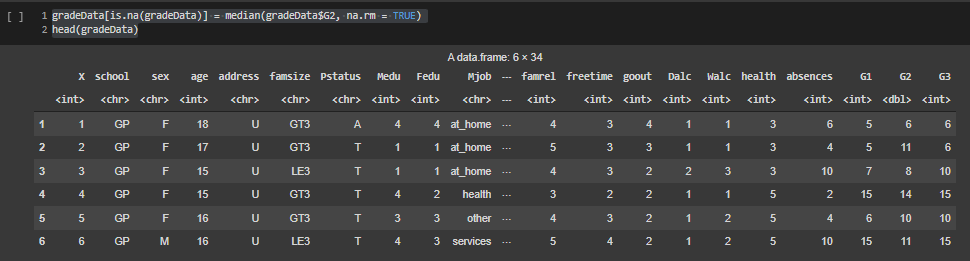
\includegraphics[scale = 1]{Images/3.PNG}
    \caption{There are 5 NA values in G2 column}
    \label{fig:summary}
\end{figure}

%%%%%%%%%%%%%%%%%%%%%%%%%%%%%%%%%%%%%%%%%%%%%%%%%%%%%%%%%%%%%%%%%%%%%%%%%%%%%%

\subsubsection{Data visualization}
\vspace{0.4cm}
\textbf{1.2.3.1. Transformation} \\ \newline
\addcontentsline{toc}{subsubsection}{\hspace{1cm}1.2.3.1. Transformation}
To utilize R program to calculate, all factors or values from the dataset must be transferred to numeric type. Before the transformation process is coded, several implies are established for thorough understanding.
\begin{itemize}
    \item School: GP = 0 \hspace{5cm} Sex: Female = 1 
    \item School: MS = 1 \hspace{5cm} Sex: Male = 0\\  
    \item Address: U = 0 \hspace{5cm} Famsize: GT3 = 0
    \item Address: R = 1 \hspace{5cm} Famsize: LE3 = 1 \\
    \item Pstatus: A = 0
    \item Pstatus: T = 1 \\
    \item Jobs: at\_home = 0 \hspace{4.52cm} Reason: course = 0
    \item Jobs: services = 1 \hspace{4.61cm} Reason: home = 1
    \item Jobs: teacher = 2  \hspace{4.69cm} Reason: reputation = 2
    \item Jobs: health = 3   \hspace{4.84cm} Reason: other = 3 
    \item Jobs: other = 4 \\
    \item Guardian: father = 0 \hspace{4.17cm} Everything else: no = 0
    \item Guardian: mother = 1 \hspace{4.0cm} Everything else: yes = 1
    \item Guardian: other = 3 \\             
\end{itemize}
And then, converting these values to numerical values.
\begin{figure}[H]
    \centering
    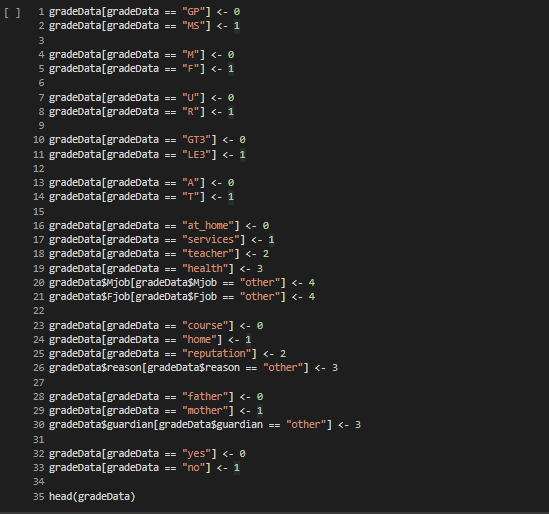
\includegraphics[scale = 1.5]{Images/4.PNG}
    \caption{Converting to numerical values}
    \label{fig:converting}
\end{figure}
Now, our dataframe is now ready for analysing.
\begin{figure}[H]
    \centering
    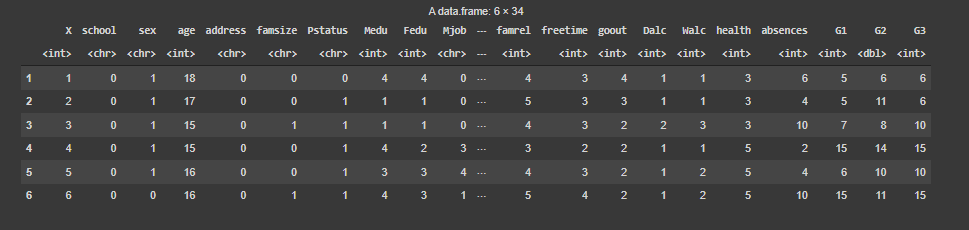
\includegraphics[scale = 1]{Images/5.PNG}
    \caption{Analysing table.}
    \label{fig:analysing}
\end{figure}

%%%%%%%%%%%%%%%%%%%%%%%%%%%%%%%%%%%%%%%%%%%%%%%%%%%%%%

\textbf{1.2.3.2. Statistics for each of the variables} \\ \newline
\addcontentsline{toc}{subsubsection}{\hspace{1cm}1.2.3.2. Statistics for each of the variables}
After the data cleaning and transformation have been done, class(gradedata and summary command is used to form all the variables into the separate table containing calculating information such as min, 1\textsuperscript{st} Qu., median, mean, 3\textsuperscript{rd} Qu., and max.
\begin{figure}[H]
    \centering
    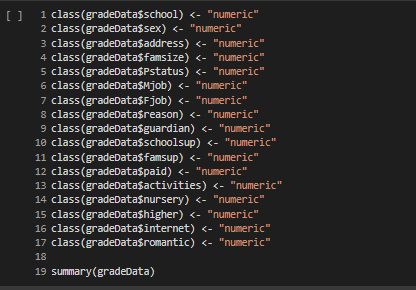
\includegraphics[scale = 1.5]{Images/6.PNG}
    \caption{Example for code.}
    \label{fig:Ex1}
\end{figure}
For example, as can be seen from the Fig. \ref{fig:details}, the description of final score G3:
\begin{itemize}
    \item The lowest score is 0.00 (Min = 0.00), the highest score is 20.00 (Max = 20.00). The range of G3 will be 20.00 - 0.00 = 20.
    \item $1^{st}$ Qu. is 8.00 shows that 25\% of students have their final score less than or equal to 8.00.
    \item Median = 11.00 shows that 50\% of students have their final score less than or equal to 11.00.
    \item $3^{rd}$ Qu. is 14.00 shows that 75\% of students have their final score less than or equal to 14.00.
    \item Mean = 10.42 shows that the average score of all 395 students is 10.42. \\
\end{itemize}
For the dummy variable sex which takes only 2 values 0 or 1, its description shows that:
\begin{itemize}
    \item Median = 1.0000, meaning that more than 50\% of values are 1.
    \item Mean = 0.5266, meaning that 52.66\% of students are female, 47.34\% of students are male. \\
\end{itemize}
Here is the description the statistics of each variable:
\begin{figure}[H]
    \centering
    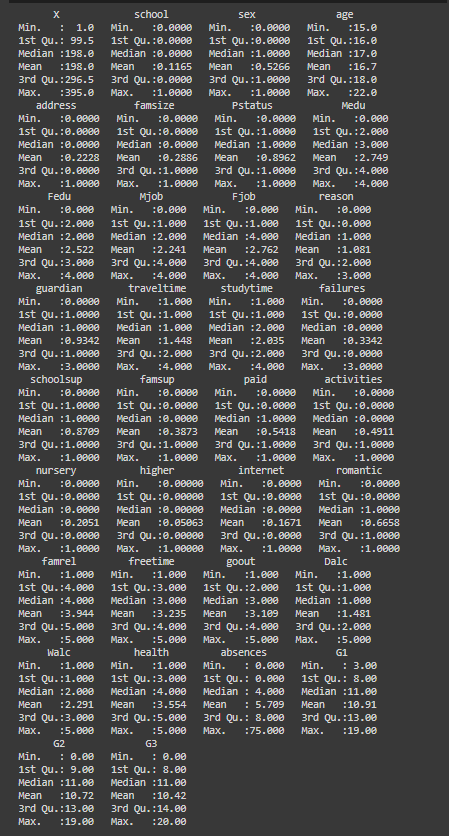
\includegraphics[scale = 1.5]{Images/7.PNG}
    \caption{The min, max, 1\textsuperscript{st} quartile, median, 3\textsuperscript{rd} quartile and the mean value of all variables are described in the result above.}
    \label{fig:details}
\end{figure}

%%%%%%%%%%%%%%%%%%%%%%%%%%%%%%%%%%%%%%%%%%%%%%%%%%%%%%

\textbf{1.2.3.3. Graphs: hist, boxplot, pair \\ \newline}
\addcontentsline{toc}{subsubsection}{\hspace{1cm}1.2.3.3. Graphs: hist, boxplot, pairs}
\textbf{1.2.3.3.a. Histogram \\ \newline} 
\addcontentsline{toc}{subsubsection}{\hspace{2cm}1.2.3.3.a. Histogram}
A histogram is a bar graph-like representation of data that buckets a range of outcomes into columns along the x-axis. The y-axis represents the number count or percentage of frequencies in the data for each column and can be used to visualize data distributions. \\ \newline
In R , we will call \textit{hist()} function to represent the histogram.
\begin{figure}[H]
    \centering
    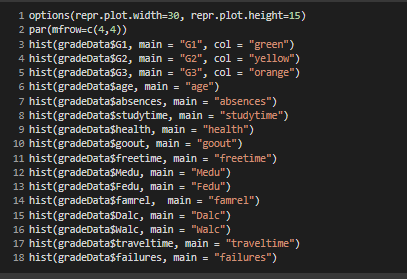
\includegraphics[scale = 1.5]{Images/8.PNG}
    \caption{The lines of code for creating histogram of each variable.}
    \label{fig:hist1}
\end{figure}
As the result, we are able to obtain the histogram of each variable.
\begin{figure}[H]
    \centering
    \begin{minipage}{0.5\textwidth}
        \centering
        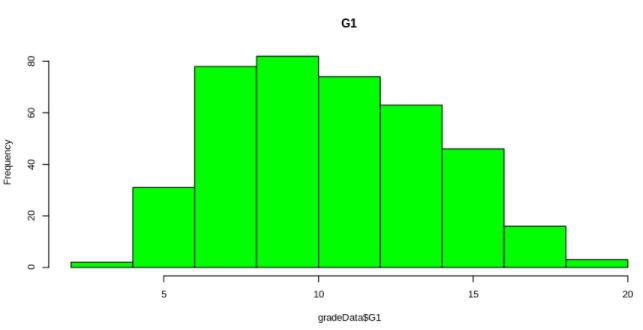
\includegraphics[width = 1\linewidth]{Images/9.PNG}
        \caption{Histogram for G1.}
        \label{fig:hist2}
    \end{minipage}%
    \begin{minipage}{0.5\textwidth}
        \centering
        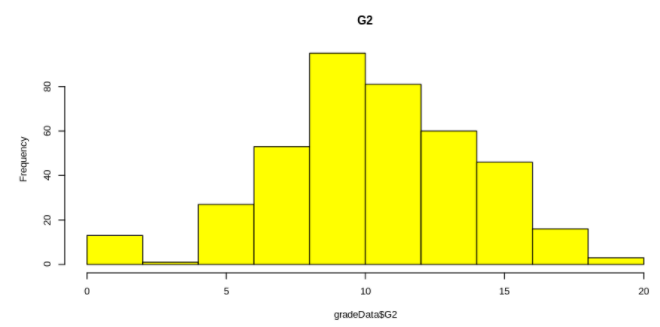
\includegraphics[width = 1\linewidth]{Images/10.PNG}
        \caption{Histogram for G2.}
        \label{fig:hist3}
    \end{minipage}
\end{figure}
\begin{figure}[H]
    \centering
    \begin{minipage}{0.5\textwidth}
        \centering
        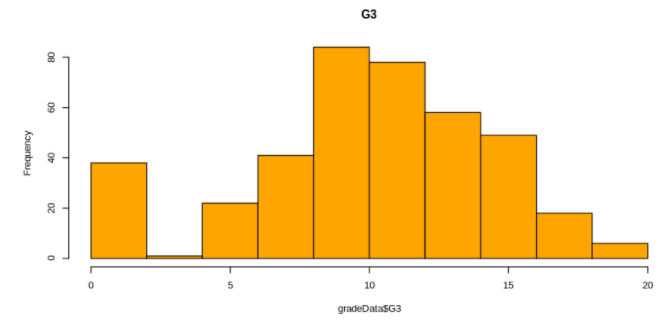
\includegraphics[width = 1\linewidth]{Images/11.PNG}
        \caption{Histogram for G3.}
        \label{fig:hist4}
    \end{minipage}%
    \begin{minipage}{0.5\textwidth}
        \centering
        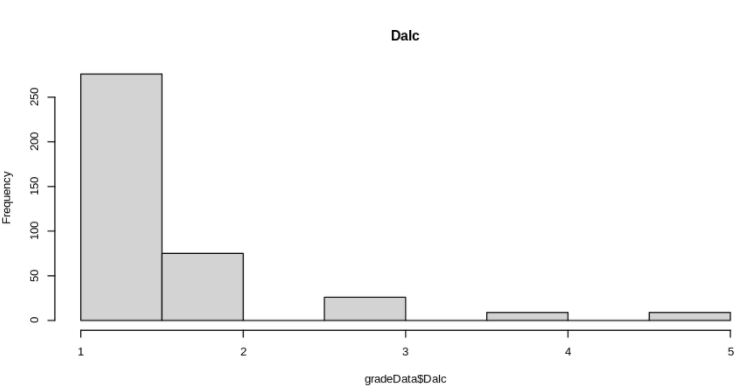
\includegraphics[width = 1\linewidth]{Images/13.PNG}
        \caption{Histogram for Dalc.}
        \label{fig:hist5}
    \end{minipage}
\end{figure}
\begin{figure}[H]
    \centering
    \begin{minipage}{0.5\textwidth}
        \centering
        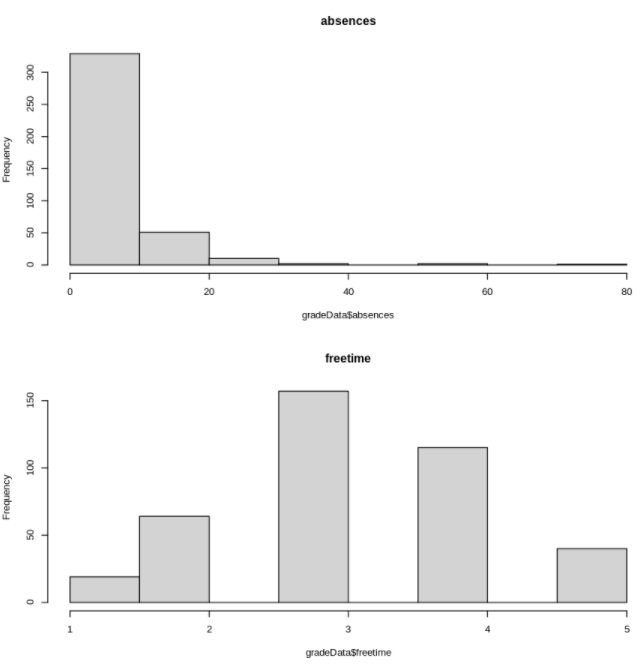
\includegraphics[width = 1\linewidth]{Images/12.PNG}
        \caption{Histogram for absences and freetime.}
        \label{fig:hist6}
    \end{minipage}%
    \begin{minipage}{0.5\textwidth}
        \centering
        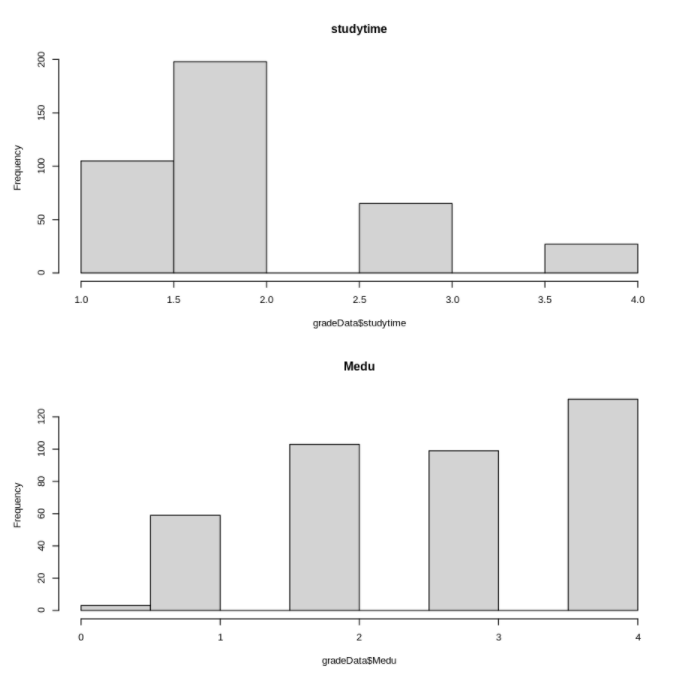
\includegraphics[width = 1.045\linewidth]{Images/15.PNG}
        \caption{Histogram for studytime and Medu.}
        \label{fig:hist8}
    \end{minipage}
\end{figure}
\begin{figure}[H]
    \centering
    \begin{minipage}{0.5\textwidth}
        \centering
        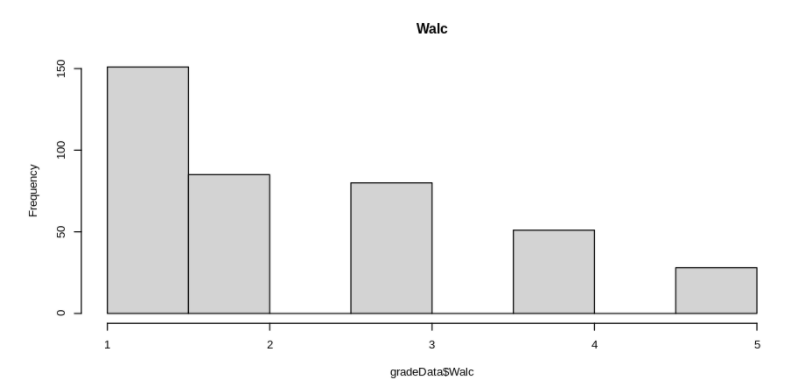
\includegraphics[width = 1\linewidth]{Images/14.PNG}
        \caption{Histogram for Walc.}
        \label{fig:hist7}
    \end{minipage}%
    \begin{minipage}{0.5\textwidth}
        \centering
        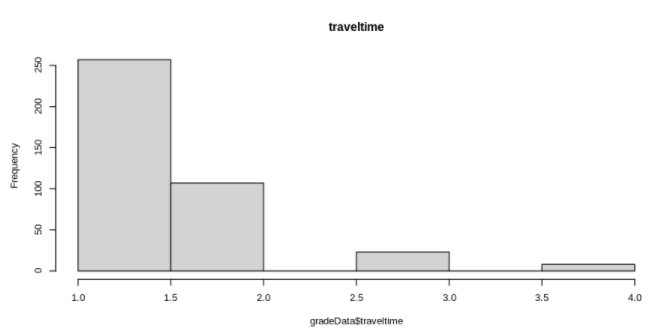
\includegraphics[width = 1\linewidth]{Images/16.PNG}
        \caption{Histogram for traveltime.}
        \label{fig:hist9}
        \end{minipage}
\end{figure}
\begin{figure}[H]
    \centering
    \begin{minipage}{0.5\textwidth}
        \centering
        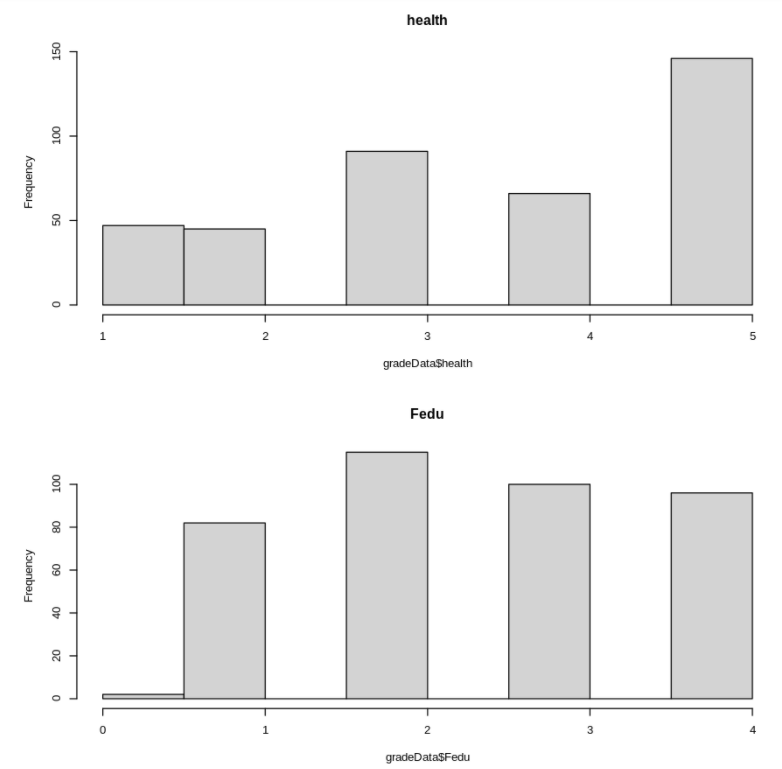
\includegraphics[width = 1.045\linewidth]{Images/17.PNG}
        \caption{Histogram for health and Fedu.}
    \label{fig:hist10}
    \end{minipage}%
    \begin{minipage}{0.5\textwidth}
        \centering
        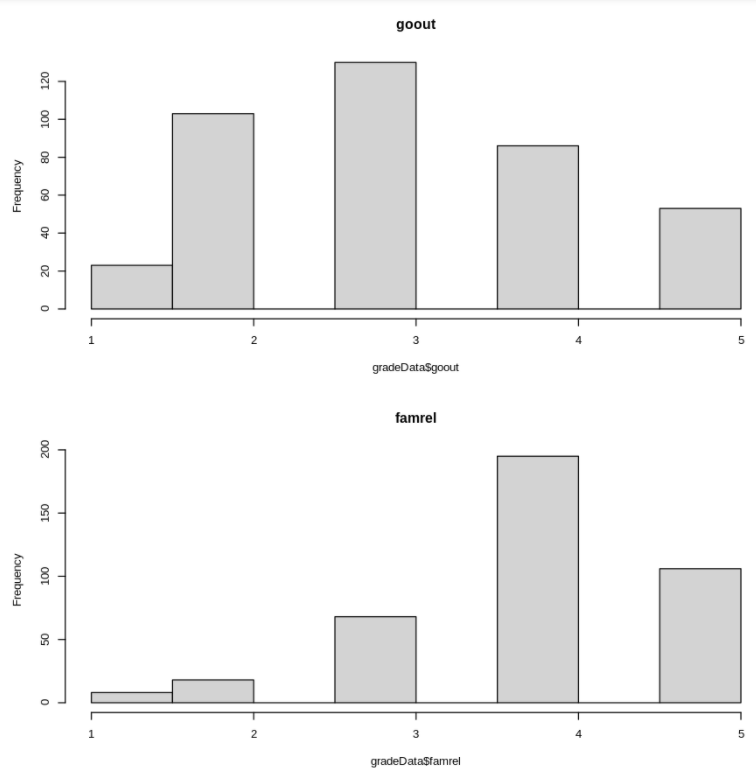
\includegraphics[width = 1\linewidth]{Images/18.PNG}
        \caption{Histogram for go out and famrel.}
        \label{fig:hist12}
        \end{minipage}
\end{figure}
\begin{figure}[H]
    \centering
    \begin{minipage}{0.5\textwidth}
        \centering
        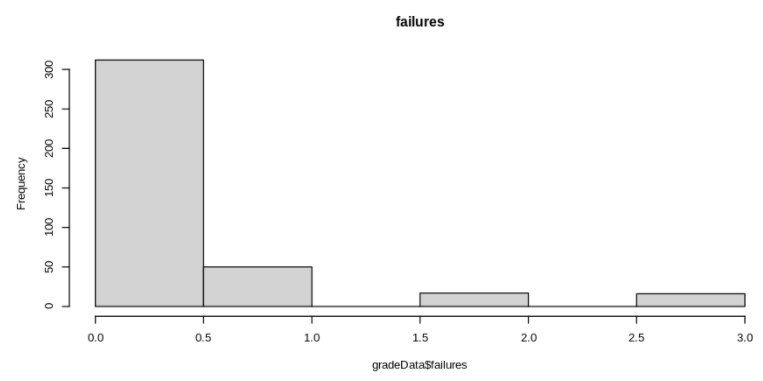
\includegraphics[width = 1\linewidth]{Images/19.PNG}
        \caption{Histogram for failures.}
        \label{fig:hist11}
    \end{minipage}%
    \begin{minipage}{0.5\textwidth}
        \centering
        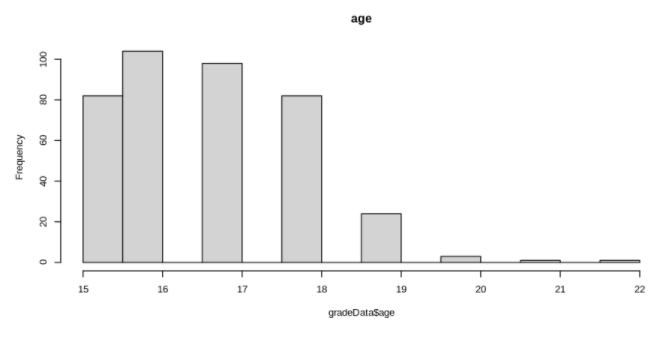
\includegraphics[width = 1\linewidth]{Images/20.PNG}
        \caption{Histogram for age.}
        \label{fig:hist13}
        \end{minipage}
\end{figure}

%%%%%%%%%%%%%%%%%%%%%%%%%%%%%%%%%%%%%%%%%

\textbf{1.2.3.3.b. Boxplot \\ \newline}
\addcontentsline{toc}{subsubsection}{\hspace{2cm}1.2.3.3.b. Boxplot}
Boxplot is a graphical representation of statistical measures like median, upper and lower quartiles, minimum and maximum data values. Thus, we will make 2 situations for comparision among G3 and the others. \\ \newline
In R, we use function \textit{boxplot()} to represent boxplot. 
\begin{enumerate}
    \item Comparing final grade G3 with G1, G2, Medu, Fedu, age, absences, studytime, health and go out. 
    \begin{figure}[H]
        \centering
        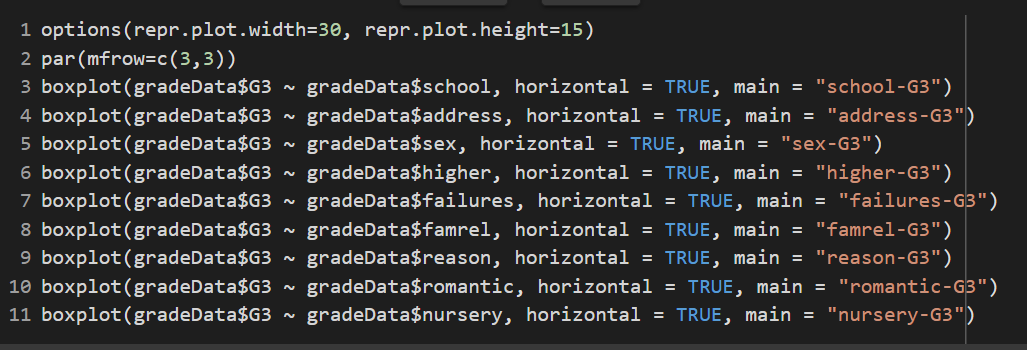
\includegraphics[scale = 0.9]{Images/21.PNG}
        \caption{The above codes are used to represent boxplot for case 1.}
        \label{fig:boxplot1}
    \end{figure}
    As the result, we are able to obtain the boxplot of each variable in case 1.
    \begin{figure}[H]
        \centering
        \begin{minipage}{0.5\textwidth}
            \centering
            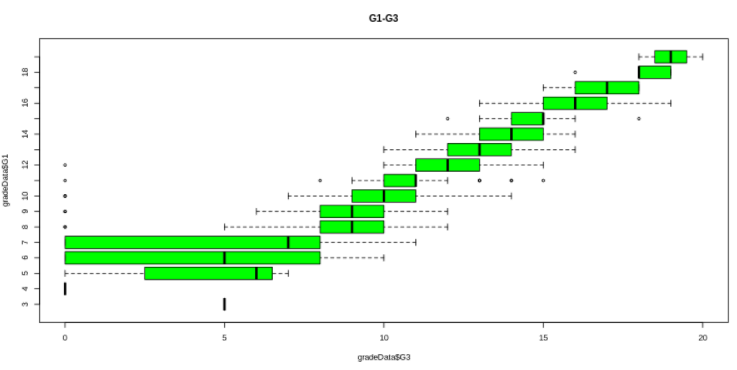
\includegraphics[width = 1\linewidth]{Images/22.PNG}
            \caption{Boxplot for G1 vs G3.}
            \label{fig:boxplot2}
        \end{minipage}%
        \begin{minipage}{0.5\textwidth}
            \centering
            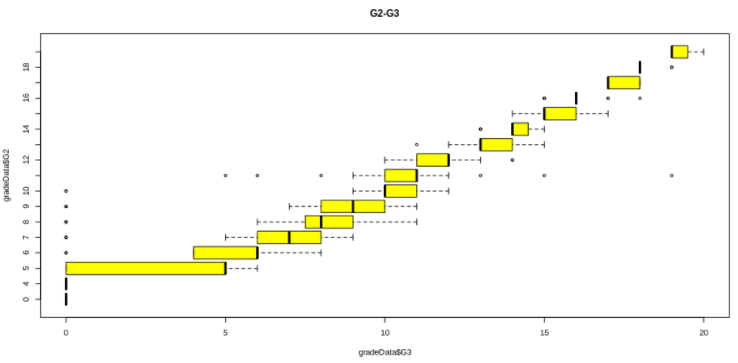
\includegraphics[width = 1\linewidth]{Images/25.PNG}
            \caption{Boxplot for G2 vs G3.}
            \label{fig:boxplot3}
        \end{minipage}
    \end{figure}
    \begin{figure}[H]
        \centering
        \begin{minipage}{0.5\textwidth}
            \centering
            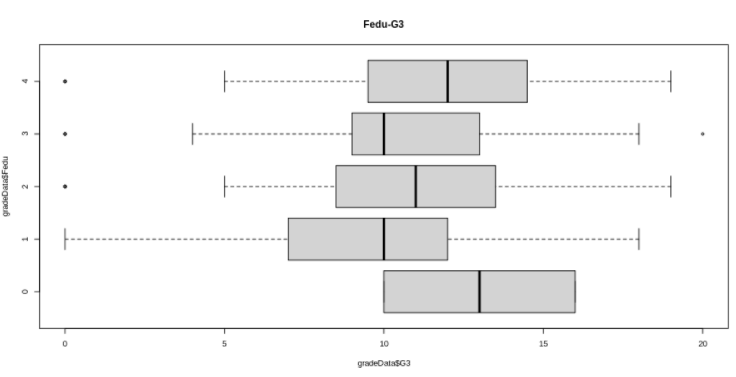
\includegraphics[width = 1\linewidth]{Images/23.PNG}
            \caption{Boxplot for Fedu vs G3.}
            \label{fig:boxplot4}
        \end{minipage}%
        \begin{minipage}{0.5\textwidth}
            \centering
            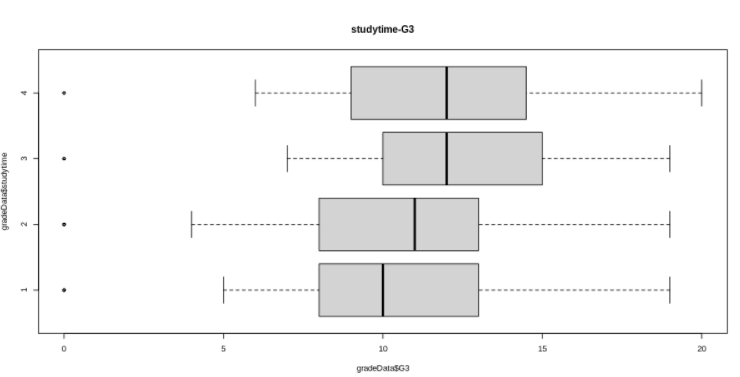
\includegraphics[width = 1\linewidth]{Images/24.PNG}
            \caption{Boxplot for studytime vs G3.}
            \label{fig:boxplot5}
        \end{minipage}
    \end{figure}
    \begin{figure}[H]
        \centering
        \begin{minipage}{0.5\textwidth}
            \centering
            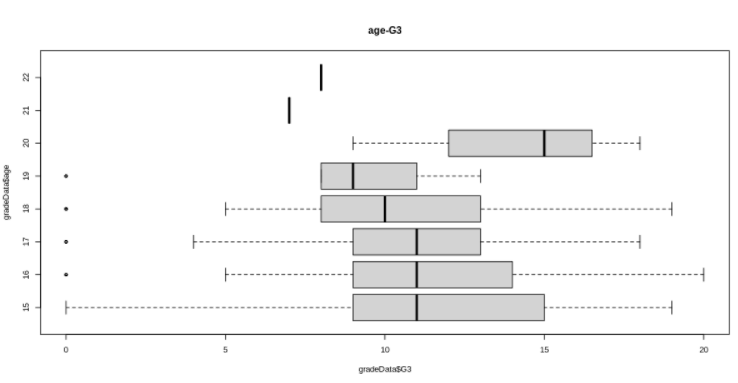
\includegraphics[width = 1\linewidth]{Images/26.PNG}
            \caption{Boxplot for age vs G3.}
            \label{fig:boxplot6}
        \end{minipage}%
        \begin{minipage}{0.5\textwidth}
            \centering
            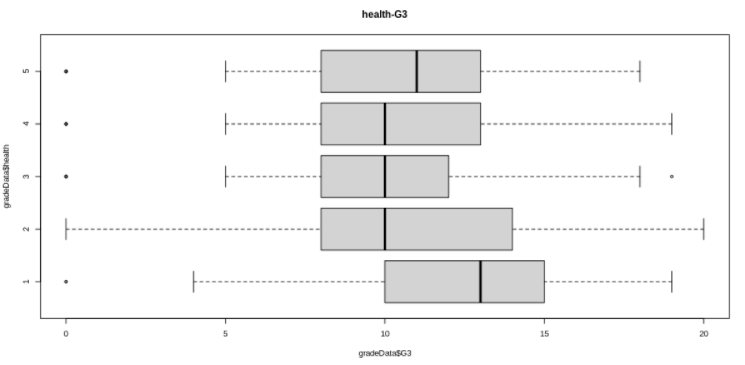
\includegraphics[width = 1\linewidth]{Images/27.PNG}
            \caption{Boxplot for health vs G3.}
            \label{fig:boxplot7}
        \end{minipage}
    \end{figure}
    \begin{figure}[H]
        \centering
        \begin{minipage}{0.5\textwidth}
            \centering
            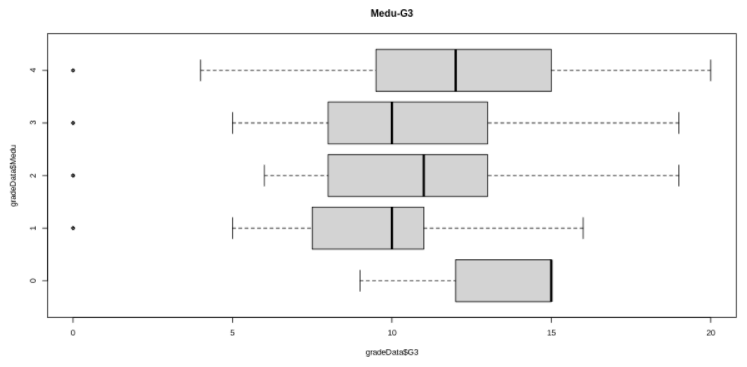
\includegraphics[width = 1\linewidth]{Images/28.PNG}
            \caption{Boxplot for Medu vs G3.}
            \label{fig:boxplot8}
        \end{minipage}%
        \begin{minipage}{0.5\textwidth}
            \centering
            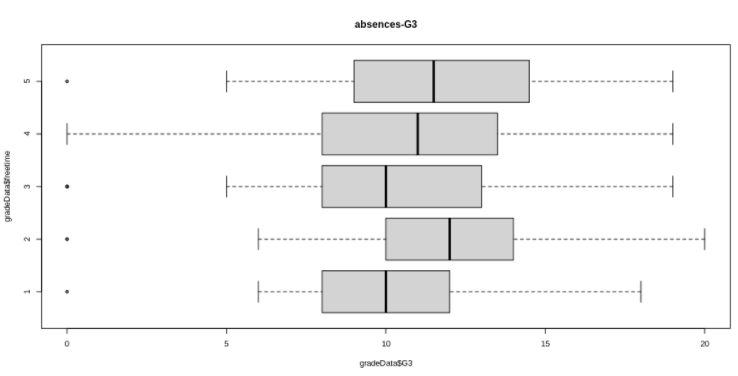
\includegraphics[width = 1\linewidth]{Images/29.PNG}
            \caption{Boxplot for absences vs G3.}
            \label{fig:boxplot9}
        \end{minipage}
    \end{figure}
    \begin{figure}[H]
        \centering
        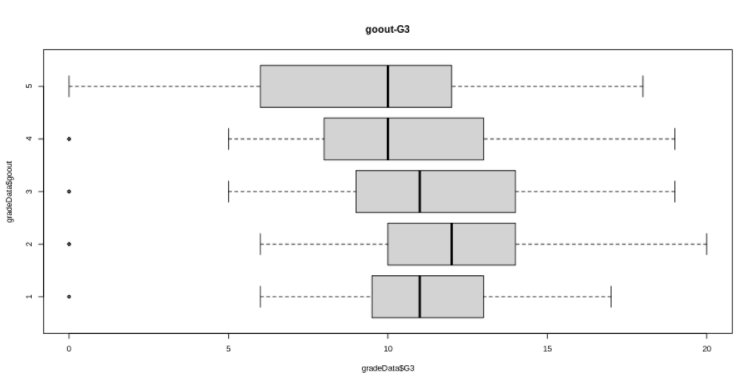
\includegraphics[width = 0.5\linewidth]{Images/30.PNG}
        \caption{Boxplot for go out vs G3.}
        \label{fig:boxplot10}
    \end{figure}
    \item Comparing final grade G3 with school, address, sex, higher, failures, famrel, reason, romantic and nursery.
    \begin{figure}[H]
        \centering
        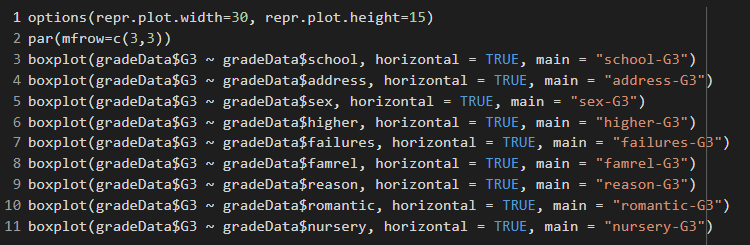
\includegraphics[scale = 1]{Images/31.PNG}
        \caption{The above codes are used to represent boxplot for case 2.}
        \label{fig:boxplot11}
    \end{figure}
    As the result, we are able to obtain the boxplot of each variable in case 2.
    \begin{figure}[H]
        \centering
        \begin{minipage}{0.5\textwidth}
            \centering
            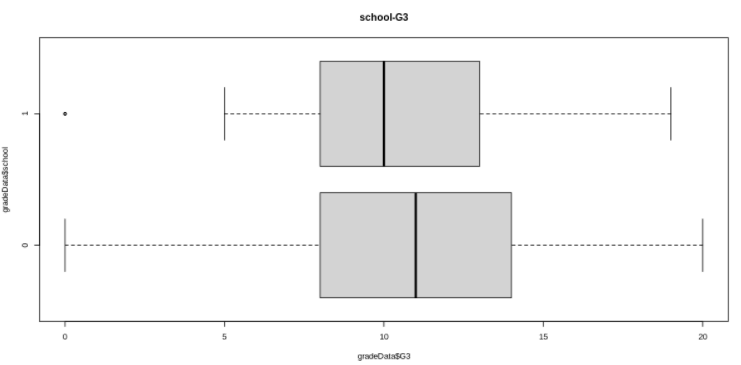
\includegraphics[width = 1\linewidth]{Images/32.PNG}
            \caption{A Boxplot for school vs G3.}
            \label{fig:boxplot12}
        \end{minipage}%
        \begin{minipage}{0.5\textwidth}
            \centering
            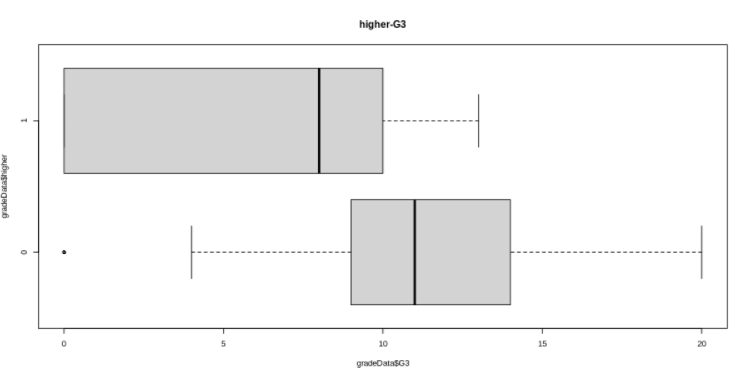
\includegraphics[width = 1\linewidth]{Images/33.PNG}
            \caption{Boxplot for higher vs G3.}
            \label{fig:boxplot13}
        \end{minipage}
    \end{figure}
    \begin{figure}[H]
        \centering
        \begin{minipage}{0.5\textwidth}
            \centering
            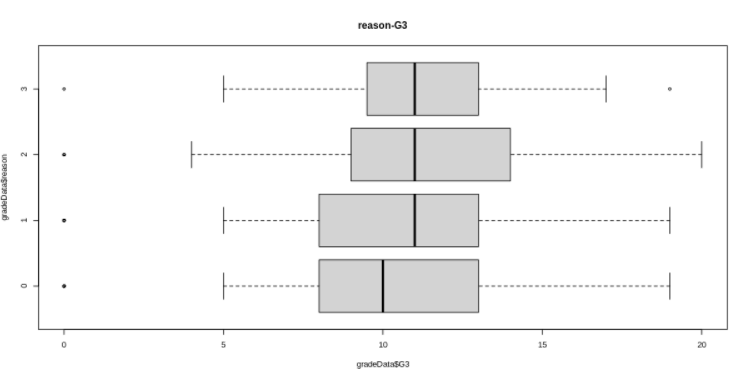
\includegraphics[width = 1\linewidth]{Images/34.PNG}
            \caption{Boxplot for reason vs G3.}
            \label{fig:boxplot14}
        \end{minipage}%
        \begin{minipage}{0.5\textwidth}
            \centering
            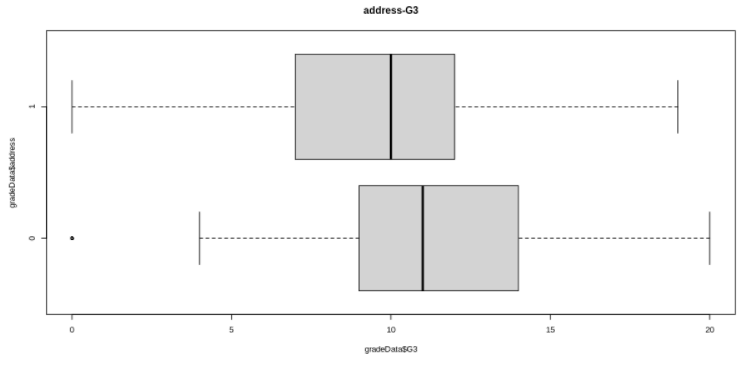
\includegraphics[width = 1\linewidth]{Images/35.PNG}
            \caption{Boxplot for address vs G3.}
            \label{fig:boxplot15}
        \end{minipage}
    \end{figure}
    \begin{figure}[H]
        \centering
        \begin{minipage}{0.5\textwidth}
            \centering
            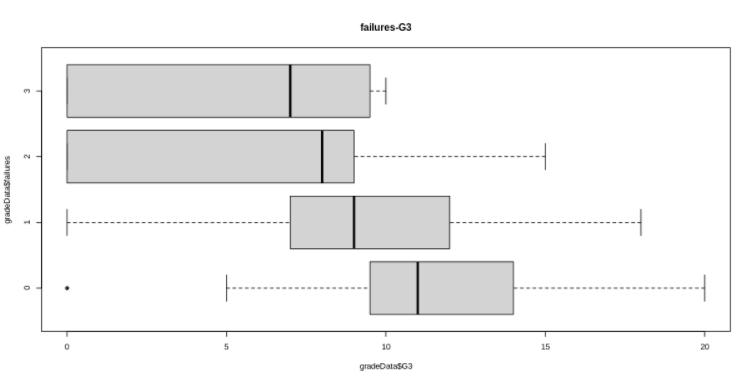
\includegraphics[width = 1\linewidth]{Images/36.PNG}
            \caption{Boxplot for failures vs G3.}
        \label{fig:boxplot16}
        \end{minipage}%
        \begin{minipage}{0.5\textwidth}
            \centering
            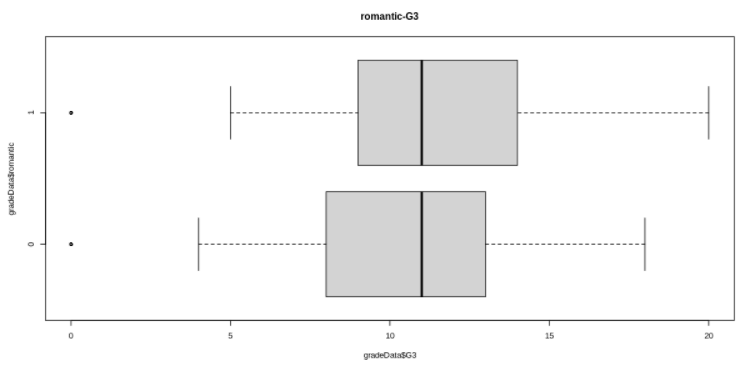
\includegraphics[width = 1\linewidth]{Images/37.PNG}
            \caption{Boxplot for romantic vs G3.}
        \label{fig:boxplot17}
        \end{minipage}
    \end{figure}
    \begin{figure}[H]
        \centering
        \begin{minipage}{0.5\textwidth}
            \centering
            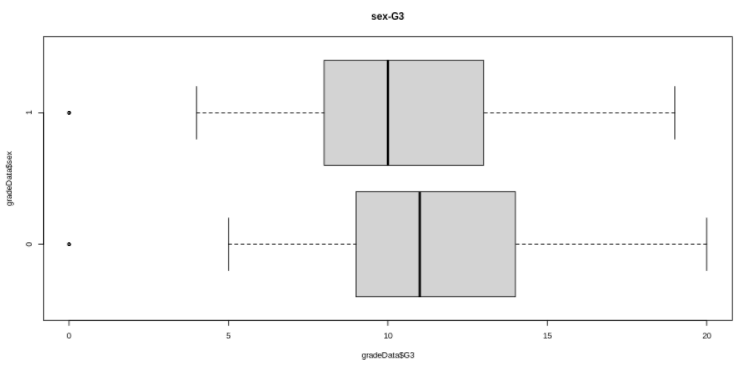
\includegraphics[width = 1\linewidth]{Images/38.PNG}
            \caption{Boxplot for sex vs G3.}
            \label{fig:boxplot18}
        \end{minipage}%
        \begin{minipage}{0.5\textwidth}
            \centering
            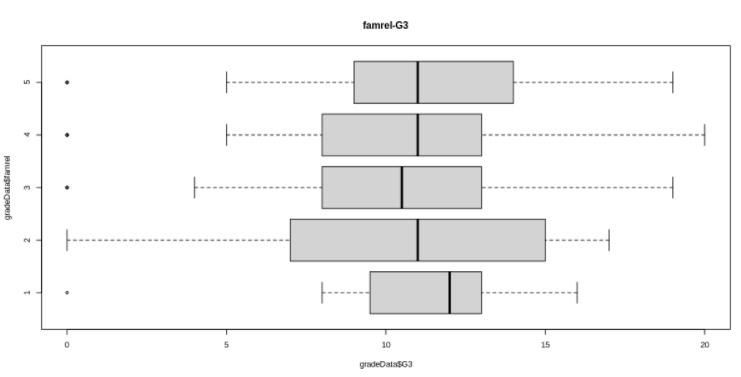
\includegraphics[width = 1\linewidth]{Images/39.PNG}
            \caption{Boxplot for famrel vs G3.}
            \label{fig:boxplot19}
        \end{minipage}
    \end{figure}
    \begin{figure}[H]
        \centering
        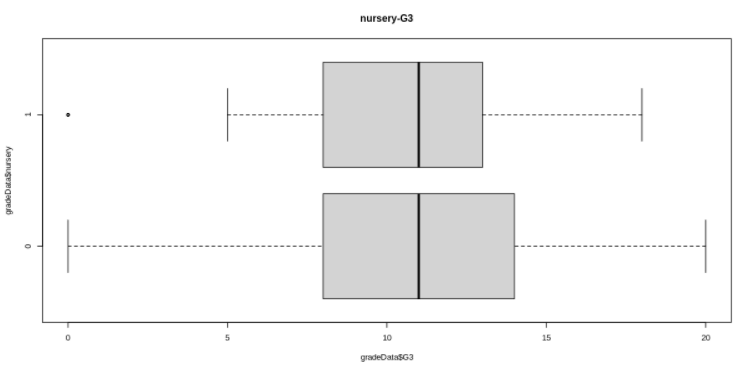
\includegraphics[width = 0.5\linewidth]{Images/40.PNG}
        \caption{Boxplot for nursery vs G3.}
        \label{fig:boxplot20}
    \end{figure}
\end{enumerate}

%%%%%%%%%%%%%%%%%%%%%%%%%%%%%%%%%%%%%%%%%%%%%%%%%

\textbf{1.2.3.3.c. Pairs \\ \newline}
\addcontentsline{toc}{subsubsection}{\hspace{2cm}1.2.3.3.c. Pairs}
The \textit{pairs} command in R function returns a plot matrix, consisting of scatterplots for each variable-combination of a data frame. In other words, using it to show the statistical relationship between variables (failures, age, higher, absences, famrel, Medu, Fedu, G1, G2 and G3).
\begin{figure}[H]
    \centering
    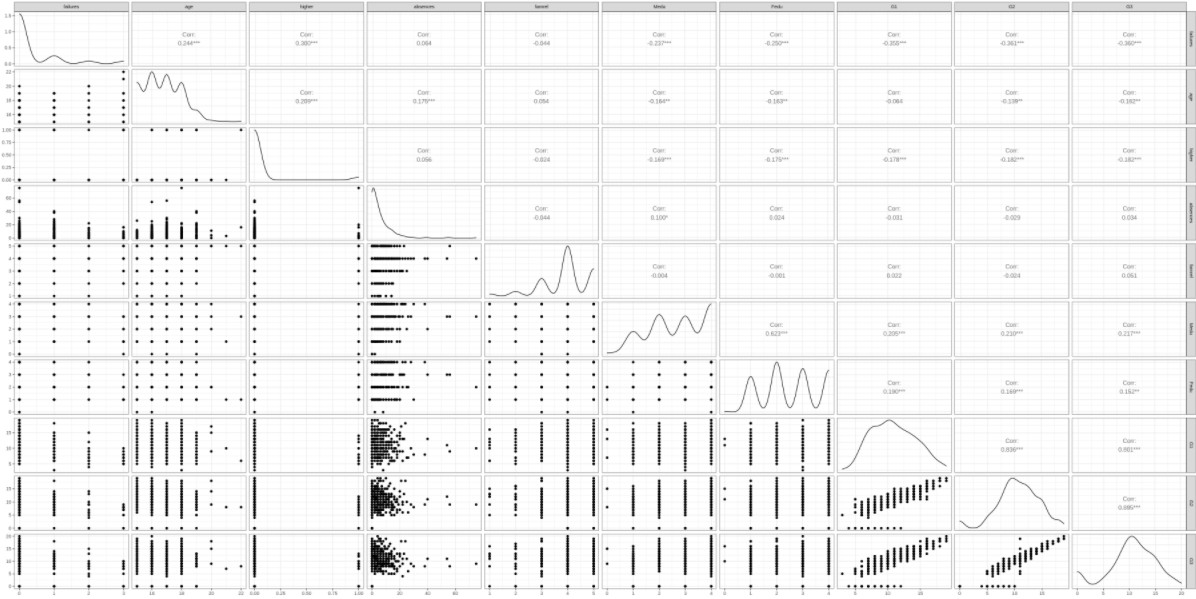
\includegraphics[scale = 0.8]{Images/42.PNG}
    \caption{Some linearity can be seen between pairs of variables, such as G1 and G3, or G2 and G3.}
    \label{fig:pairs2}
\end{figure}
\begin{figure}[H]
    \centering
    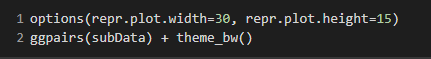
\includegraphics[scale = 1.5]{Images/41.PNG}
    \caption{The basic R syntax for the pairs command.}
    \label{fig:pairs1}
\end{figure}

%%%%%%%%%%%%%%%%%%%%%%%%%%%%%%%%%%%%%%%%

\textbf{1.2.3.4. Fitting linear regression models \\ \newline}
\addcontentsline{toc}{subsubsection}{\hspace{1cm}1.2.3.4. Fitting linear regression models}
First, using below command to confirm that G3 is a function of the other
values and \textit{data} = \textit{grade} confirm that R has to compute on dataset called grade.
\begin{figure}[H]
    \centering
    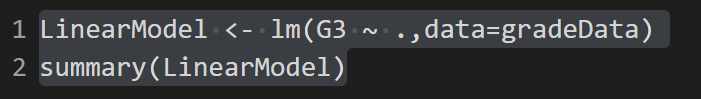
\includegraphics[scale = 0.8]{Images/43.PNG}
    \caption{Example for code.}
    \label{fig:linear1}
\end{figure}
Here for the result
\begin{figure}[H]
    \centering
    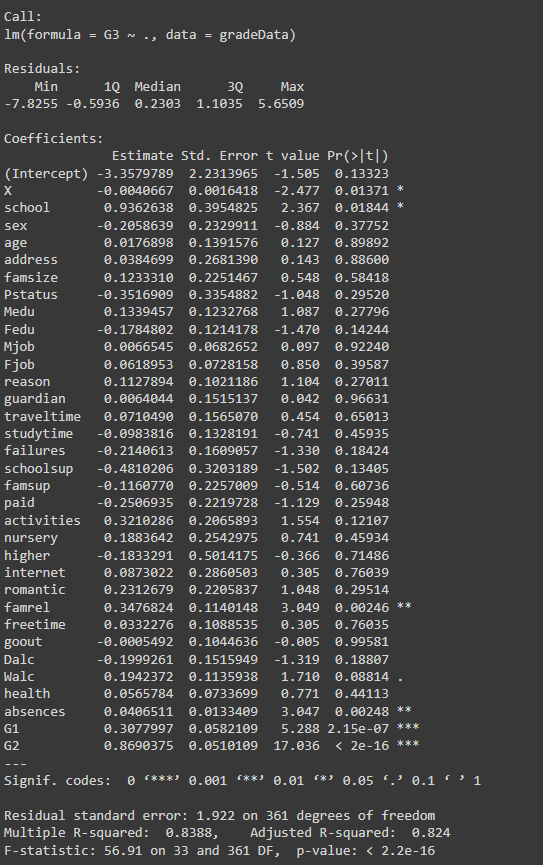
\includegraphics[scale = 1]{Images/44.PNG}
    \caption{Result of the codes.}
    \label{fig:linear2}
\end{figure}
Based on p-value, constructing 6 models more by eliminating one by one variable from the low p-value to the worst.
\begin{figure}[H]
    \centering
    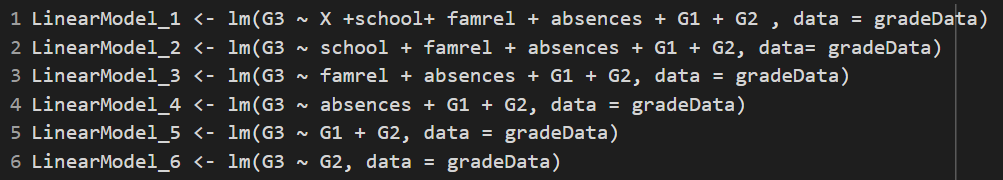
\includegraphics[scale = 0.8]{Images/45.PNG}
    \caption{Example for the codes.}
    \label{fig:linear3}
\end{figure}
Then, by \textit{anova} command, the comparison between regression models are built.
\begin{figure}[H]
    \centering
    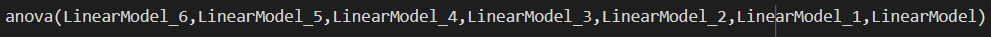
\includegraphics[scale = 0.8]{Images/46.PNG}
    \caption{Example for the codes.}
    \label{fig:linear4}
\end{figure}
Now, the result will be taken.
\begin{figure}[H]
    \centering
    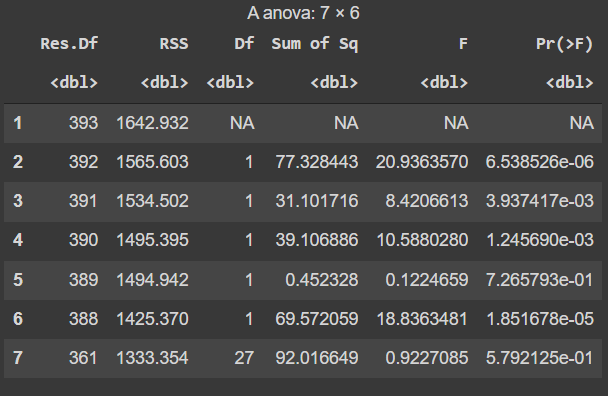
\includegraphics[scale = 1]{Images/47.PNG}
    \caption{The results of the code.}
    \label{fig:linear5}
\end{figure}
Observing the Anova data table from the model 1 to 7, the result has illustrated that the model 2 seems to be the finest model to be built a fitting linear regression model compared to other models because of the p-value (the model 2 has smallest value, p2 $\sim$ 0.019).
\begin{figure}[H]
    \centering
    \includegraphics[scale = 1.3]{Images/48.PNG}
    \caption{Model 2.}
    \label{fig:linear6}
\end{figure}
Then, having the fitting model below.
\begin{figure}[H]
    \centering
    \includegraphics[scale = 1.3]{Images/49.PNG}
    \caption{The fitting model.}
    \label{fig:linear7}
\end{figure}
As the result, we have the formula: \hspace{0.5cm} \textbf{G3} = -3.77114 + 0.93638 × \textit{G2} + 0.23115 × \textit{G1} + 0.35501 × \textit{famrel} + 0.03726 × \textit{absences} + 0.10628 × \textit{school1}. \\ \newline \newline
Following that, plotting that model.
\begin{mdframed}[leftline=false,rightline=false,backgroundcolor=magenta!10,nobreak=true]
    \begin{minted}[linenos,breaklines,breaksymbolleft=,obeytabs=true,tabsize=2]{R}
plot(LinearModel_2)
    \end{minted}
\end{mdframed}
\begin{figure}[H]
    \centering
    \includegraphics[width = 1.1\linewidth]{Images/50.PNG}
    \caption{Residuals vs Fitted.}
    \label{fig:linear8}
\end{figure}
\begin{figure}[H]
    \centering
    \includegraphics[width = 1.1\linewidth]{Images/51.PNG}
    \caption{Normal Q-Q.}
    \label{fig:linear9} 
\end{figure}
\begin{figure}[H]
    \centering
    \includegraphics[width = 1.1\linewidth]{Images/52.PNG}
    \caption{Scale-Location.}
    \label{fig:linear10}
\end{figure}
\begin{figure}[H]
    \centering
    \includegraphics[width = 1.1\linewidth]{Images/54.PNG}
    \caption{Residuals vs Leverage.}
    \label{fig:linear11}
\end{figure}

%%%%%%%%%%%%%%%%%%%%%%%%%%%%%%%%%%%%%%%%%

\subsubsection{Predictions}
\vspace{0.4cm}
\textbf{1.2.4.1. Evaluation} \\ \newline
\addcontentsline{toc}{subsubsection}{\hspace{1cm}1.2.4.1. Evaluation}
First, in order to evaluate whether those students passed or failed based on
final grade, the condition order: \textit{if their final grade is not less than 10, they are passed}; which is used to \textit{evaluate}. After that step, the prediction data also is built as the same function above but predict\_G3.
\begin{figure}[H]
    \centering
    \begin{minipage}{0.5\textwidth}
        \centering
        \includegraphics[width = 1\linewidth]{Images/55.PNG}
        \caption{The code for evaluate.}
        \label{fig:prediction1}
    \end{minipage}%
    \begin{minipage}{0.5\textwidth}
        \centering
        \includegraphics[width = 0.34\linewidth]{Images/56.PNG}
        \caption{The result of evaluate.}
        \label{fig:prediction2}
    \end{minipage}
\end{figure}
\begin{figure}[H]
    \centering
    \begin{minipage}{0.5\textwidth}
        \centering
        \includegraphics[width = 1\linewidth]{Images/57.PNG}
        \caption{The code for Predict\_G3.}
        \label{fig:prediction3}
    \end{minipage}%
    \begin{minipage}{0.5\textwidth}
        \centering
        \includegraphics[width = 0.34\linewidth]{Images/58.PNG}
        \caption{The result of Predict\_G3.}
        \label{fig:prediction4}
    \end{minipage}
\end{figure}
The percent error for students who failed is $\frac{185 - 130}{130}$ \textcolor{blue}{x} $100\% = 42.31\% $. \\ \newline
The percent error for students who passed is $\frac{265 - 210}{265}$ \textcolor{blue}{x} $100\% = 20.75\% $. \\ \newline

%%%%%%%%%%%%%%%%%%%%%%%%%%%%%%%%

\vspace{0.4cm}
\textbf{1.2.4.2. Prediction a new data} \\ \newline
\addcontentsline{toc}{subsubsection}{\hspace{1cm}1.2.4.2. Prediction a new data}
First, creating a data frame to predict the final grade. As below, the new data frame is given as an example
\begin{figure}[H]
    \centering
    \includegraphics[scale = 1.3]{Images/59.PNG}
    \label{fig:prediction5}
\end{figure}
Then, using \textit{predict} command to compute G3 (final grade) from the others
factor in the data frame.
\begin{figure}[H]
    \centering
    \includegraphics[scale = 1.5]{Images/60.PNG}
    \label{fig:prediction6}
\end{figure}
And using \textit{round} command to round the result.
\begin{figure}[H]
    \centering
    \includegraphics[scale = 1.5]{Images/61.PNG}
    \label{fig:prediction7}
\end{figure}
Then, we will have the result.
\begin{figure}[H]
    \centering
    \includegraphics[scale = 1.5]{Images/62.PNG}
    \label{fig:prediction8}
\end{figure}
Finally, the final result computed by R is \textbf{11.4671}.

%%%%%%%%%%%%%%%%%%%%%%%%%%%%%%%%%%%%%%%%%%%%%%%%%%%%%%%%%%%%%%%%%%%%%%%%%%%%
%%%%%%%%%%%%%%%%%%%%%%%%%%%%%%%%%%%%%%%%%%%%%%%%%%%%%%%%%%%%%%%%%%%%%%%%%%%%

\newpage
\section{\textcolor{blue}{Activity 2}}
\noindent
\subsection{Problem} 
\vspace{0.4cm}
For this activity, we use a dataset that approaches the influence of parents educational level in guiding children to prepare homework to take the exam. The data contains several factors that are considered to influence the average score of student.\\ \newline
There are 3 attributes that will be focused on in this activity:
\begin{itemize}
    \item \textit{ParentLevel}: The education level of each student (binary: \textcolor{blue}{0} - \textbf{\textit{bachelor's degree}}, \textbf{\textit{master's degree}}, \textbf{\textit{associate's degree}} or \textcolor{blue}{1} - \textbf{\textit{high school}}, \textbf{\textit{some college}}, \textbf{\textit{some highe school}}). 
    \item \textit{TestPreparation}: The preparation before having a test (binary: \textcolor{blue}{0} - \textbf{\textit{completed}} or \textcolor{blue}{1} - \textbf{\textit{none}}).
    \item \textit{AverageScore}: Student's average score (numeric: \textbf{0} - \textbf{100})
\end{itemize}
We want to know whether the education level of parents and the preparation before having a test affects the average score of student or not.
\subsection{Solution} 
\vspace{0.4cm}
\subsubsection{Import Data}
\vspace{0.4cm}
First, we will install and calling necessary library. After that, reading dataset and choosing needed elements will be the next step.
\begin{figure}[H]
    \centering
    \begin{minipage}{0.5\textwidth}
        \centering
        \includegraphics[width = 1.7\linewidth]{Images/Activity2/1.png}
        \caption{Installing and calling.}
        \label{fig:import1}
    \end{minipage}%
    \begin{minipage}{0.5\textwidth}
        \centering
        \includegraphics[width = 1\linewidth]{Images/Activity2/2.png}
        \caption{Read and choose elements.}
        \label{fig:import2}
    \end{minipage}
\end{figure}
Select necessary variables, which are "ParentLevel", "TestPreparation" and "AverageScore".
\begin{figure}[H]
    \centering 
    \includegraphics[scale = 0.7]{Images/Activity2/3.png}
    \caption{There are 1000 students that the experiment be conducted on}
    \label{fig:import3}
\end{figure}

%%%%%%%%%%%%%%%%%%%%%%%%%%%%%%%%%%%%%%%%%%%%%%%%%%%%%%%%%%%%%%%%%%%%%%%%%

\subsubsection{Data Visualizaion}
\vspace{0.4cm}
\textbf{2.2.2.1. Transformation} \\ \newline
\addcontentsline{toc}{subsubsection}{\hspace{1cm}2.2.2.1. Transformation}
To utilize R program to calculate, all factors or values from the dataset must be transferred to
numeric type. Before the transformation process is coded, several implies are established for thorough
understanding in order to convert these values to numerical values.
\begin{figure}[H]
    \centering
    \includegraphics[scale = 0.7]{Images/Activity2/4.png}
    \caption{Converting to numerical values}
    \label{fig:Trans1}
\end{figure}
And then, converting to specific value to plot the paragraph
\begin{figure}[H]
    \centering
    \begin{minipage}{0.5\textwidth}
        \centering
        \includegraphics[width = 1.3\linewidth]{Images/Activity2/6.png}
        \caption{Converting to specific value.}
        \label{fig:trans3}
    \end{minipage}%
    \begin{minipage}{0.5\textwidth}
        \centering
        \includegraphics[width = 1.2\linewidth]{Images/Activity2/5.png}
        \caption{Example for code.}
        \label{fig:trans2}
    \end{minipage}
\end{figure}


%%%%%%%%%%%%%%%%%%%%%%%%%%%%%%%%%%%%%%%%%%%%%%%%%%%%%%%%%%

\textbf{2.2.2.2. Visualization} \\ \newline
\addcontentsline{toc}{subsubsection}{\hspace{1cm}2.2.2.2. Visualization}
The frequency of each parent level line type is plotted as followed:
\begin{figure}[H]
    \centering
    \begin{minipage}{0.5\textwidth}
        \centering
        \includegraphics[width = 0.8\linewidth]{Images/Activity2/8.png}
        \caption{Levels of parents.}
        \label{fig:vis1}
    \end{minipage}%
    \begin{minipage}{0.5\textwidth}
        \centering
        \includegraphics[width =1.5\linewidth]{Images/Activity2/7.png}
        \caption{Example for code.}
        \label{fig:vis2}
    \end{minipage}
\end{figure}
And, the same for status of preparation
\begin{figure}[H]
    \centering
    \begin{minipage}{0.5\textwidth}
        \centering
        \includegraphics[width = 0.8\linewidth]{Images/Activity2/10.png}
        \caption{Status of Preparation.}
        \label{fig:trans3}
    \end{minipage}%
    \begin{minipage}{0.5\textwidth}
        \centering
        \includegraphics[width = 1.2\linewidth]{Images/Activity2/9.png}
        \caption{Example for code.}
        \label{fig:trans2}
    \end{minipage}
\end{figure}
After that, we will retransform data to integer to plot against different combinations.
\begin{figure}[H]
    \centering
    \includegraphics[scale = 0.7]{Images/Activity2/11.png}
    \caption{Example for codes.}
    \label{fig:Trans4}
\end{figure}
Then, receptivity rating is plotted separately against different combinations of ParentLevel and Preparation.
\begin{figure}[H]
    \centering
    \begin{minipage}{0.5\textwidth}
        \centering
        \includegraphics[width = 1\linewidth]{Images/Activity2/12.png}
    \end{minipage}%
    \begin{minipage}{0.5\textwidth}
        \centering
        \includegraphics[width = 1\linewidth]{Images/Activity2/13.png}
    \end{minipage}
\end{figure}
\begin{figure}[H]    
    \begin{minipage}{0.5\textwidth}
        \centering
        \includegraphics[width = 1\linewidth]{Images/Activity2/14.png}
    \end{minipage}%
    \begin{minipage}{0.5\textwidth}
        \centering
        \includegraphics[width = 1\linewidth]{Images/Activity2/15.png}
    \end{minipage}
\end{figure}
\begin{figure}[H]   
    \begin{minipage}{0.5\textwidth}
        \centering
        \includegraphics[width = 1\linewidth]{Images/Activity2/16.png}
    \end{minipage}%
    \begin{minipage}{0.5\textwidth}
        \centering
        \includegraphics[width = 1\linewidth]{Images/Activity2/17.png}
    \end{minipage}
\end{figure}
\begin{figure}[H]
    \centering
    \includegraphics[width = 0.7\linewidth]{Images/Activity2/18.png}
    \caption{Example for code.}
    \label{fig:trans5}
\end{figure}
\begin{figure}[H]
    \centering
    \includegraphics[width = 1.1\linewidth]{Images/Activity2/19.png}
    \caption{Different combinations of ParentLevel and Preparation.}
    \label{fig:trans6}
\end{figure}

%%%%%%%%%%%%%%%%%%%%%%%%%%%%%%%%%%%%%%%%%%%%%%%%%%%%%%%%%%%%%%%%%%%%5%%%%

\subsubsection{Model of Variances Analysis}
\vspace{0.4cm}
At the significance level $\alpha$ = 5\%, we test the 3 following hypotheses
\begin{itemize}
    \item \textit{$H_{0a}$}: Different types of ParentLevel lines do not affect the rating of average student's score (Main effect for ParentLevel Line).
    \item \textit{$H_{0b}$}: The preparation of test does not affect the rating of average student's score (Main effect for TestPreparation).
    \item \textit{$H_{0c}$}: There is no interaction between types of ParentLevel lines and TestPreparation on the average student's score (Interaction effect).
\end{itemize}
Respectively, we have 3 alternative hypotheses:
\begin{itemize}
    \item \textit{$H_{1a}$}: Different types of ParentLevel lines affect the rating of average student's score.
    \item \textit{$H_{1b}$}: THe preparation of test affects the rating of average student's score.
    \item \textit{$H_{1c}$}: There is an interaction between types of ParentLevel lines and TestPreparation on the average student's score.
\end{itemize}
Since we are analyzing the effects of 2 independent variables: ParentLevel Lines and TestPreparation on 1 dependent variable, which is the average score of student, Two-Way ANOVA is applied for the model of variances. \\ \newline
To test Two-Way ANOVA with both main effects and interaction effect, we used aov() function
with command Receptivity $\sim$ ParentLevel $*$ TestPreparation where "$*$" indicates interaction. \\ \newline
Here for the codes:
\begin{figure}[H]
    \centering
    \includegraphics[scale = 0.7]{Images/Activity2/20.png}
    \caption{Example for code.}
    \label{fig:analysis1}
\end{figure}
Following is the result:
\begin{figure}[H]
    \centering
    \includegraphics[scale = 0.7]{Images/Activity2/21.png}
    \caption{The result of code.}
    \label{fig:analysis2}
\end{figure}
As can be seen from the image, the Sum Squares, Mean Squares, F values and p values for 3 hypothesis tests were shown in the first 3 rows respectively:
\begin{itemize}
    \item The first row tests the effect of ParentLevel Line types on the average score of student. Because p-value (6.42e-09) is much smaller than $\alpha$ (0.05), \textit{$H_{0a}$} is rejected.
    \item The second row tests the effect of TestPrepration on the average score of stuent. As p-value (< 2e-16) is significantly smaller than $\alpha$ (0.05), \textit{$H_{0b}$} is rejected.
    \item The third row testes the interaction effect between ParentLevel Line types and TestPreparation. Since value (0.93) is greater than $\alpha$ (0.05), \textit{$H_{0c}$} is not rejected. \\
\end{itemize}
\textbf{Conclusion}: With significance level $\alpha$ = 0.05, we have evidence to confirm that different ParentLevel types affects the average student's score and there does not have an interaction between types of ParentLevel lines and TestPreparation on the average student's score.

%%%%%%%%%%%%%%%%%%%%%%%%%%%%%%%%%%%%%%%%%%%%%%%%%%%%%%%%%%%%%%%%%%%%%%

\subsubsection{Model adequacy checking}
\vspace{0.4cm}
ANOVA assumes that observations are independent normally distributed and variances between groups are homogeneous. The assumption of independence can be guaranteed, as the experiments are conducted randomly from students. Now we need to check for the homogeneity of variance and the normality assumptions to see whether our model is valid or not. \\ \newline

%%%%%%%%%%%%%%%%%%%%%%%%%%%%%%%%%%%%%%%%%%%%%%%%%%%%%%%%%%%%%%%%%%%%%%%

\textbf{2.2.4.1. Homogeneity of variances assumption} \\ \newline
\addcontentsline{toc}{subsubsection}{\hspace{1cm}2.2.4.1. Homogeneity of variances assumption}
There are 2 levels of “TestPreparation”, 2 levels of “ParentLevel”, in total there are 4 groups of combination. \\ \newline 
Here for the codes: 
\begin{figure}[H]
    \centering
    \includegraphics[scale = 0.6]{Images/Activity2/22.png}
    \caption{The example of code.}
    \label{fig:model1}
\end{figure}
The residual plots for each group:
\begin{figure}[H]
    \centering
    \includegraphics[scale = 0.7]{Images/Activity2/23.png}
    \caption{The result of codes.}
    \label{fig:model2}
\end{figure}
Although there are some outliers such as point 60, the variances seem to be the same between groups. The data variance of 2 middle groups may be slightly smaller but it is acceptable. No strange patterns found in the residual plots, indicating the homogeneity of variance. \\ \newline
Levene’s test can also be used to check the assumption of constant variances, by using function leveneTest from the package \textit{Car}:
\begin{figure}[H]
    \centering
    \includegraphics[scale = 0.7]{Images/Activity2/24.png}
    \caption{The example of codes.}
    \label{fig:model3}
\end{figure}
From the output above we can see that p-value is much larger than the significance level of
0.05. This means that we do not have enough evidence to suggest that variance across groups is
statistically significant different. Therefore, we can assume the homogeneity of variances. \\ \newline

%%%%%%%%%%%%%%%%%%%%%%%%%%%%%%%%%%%%%%%%%%%%%%%%%%%%%%%%%%%%%%%%%%%%%%%%

\vspace{0.4cm}
\textbf{2.2.4.2. Normality assumption} \\ \newline
\addcontentsline{toc}{subsubsection}{\hspace{1cm}2.2.4.2. Normality assumption}
We use the normality plot of residuals (Q-Q plot), in which the quantiles of the residuals are
plotted against the quantiles of the normal distribution. If the normality assumption is correct, the plot of residuals should approximately follows a straight line. \\ \newline
Standardized residuals plot are used instead of residual plot, the result must be the same:
\begin{figure}[H]
    \centering
    \includegraphics[scale = 0.7]{Images/Activity2/25.png}
    \caption{The example of codes.}
    \label{fig:model3}
\end{figure}
\begin{figure}[H]
    \centering
    \includegraphics[scale = 0.7]{Images/Activity2/26.png}
    \caption{The result of codes.}
    \label{fig:model3}
\end{figure}
As can be seen from the image, all the points fall approximately along the reference line, so we can assume normality of our data. \\ \newline
With the normality and variances homogeneity assumptions validated, the results from our two factor ANOVA test are more reliable.

%%%%%%%%%%%%%%%%%%%%%%%%%%%%%%%%%%%%%%%%%%%%%%%%%%%%%%%%%%%%%%%%%%%%%%%%%
%%%%%%%%%%%%%%%%%%%%%%%%%%%%%%%%%%%%%%%%%%%%%%%%%%%%%%%%%%%%%%%%%%%%%%%%%

\newpage
\section{\textcolor{blue}{Bibliography}}
\begin{thebibliography}{}
\bibitem{}
Source code Activity 1 - we run directly on the google collab and then coverting to the R file. \\
\href{https://colab.research.google.com/drive/1OGkY9_N7fz-LZsCLVjzNRSqwHHbHMw4C?usp=sharing}{Available here.} 
\bibitem{}
Source code entire the assignement - we put they on the github . \\
\href{https://github.com/huyle0107/Probability-Statistic_Assignment}{Available here.}  
\bibitem{}
R-tutor.com. 2021. \textit{Estimated Multiple Regression Equation | R Tutorial}. \\
\href{http://www.r-tutor.com/elementary-statistics/multiple-linear-regression/estimated-multiple-regression-equation}{Available here} [Accessed 1 March 2021].
\bibitem{}
Advstats.psychstat.org. 2021. \textit{Relative Importance of Predictors -- Advanced Statistics using R}. \\
\href{https://advstats.psychstat.org/book/mregression/importance.php}{Available here} [Accessed 1 March 2021].
\bibitem{}
Youtube.com. 2021. \textit{R Stats: Multiple Regression - Variable Selection}. \\
\href{https://www.youtube.com/watch?v=HP3RhjLhRjY&t=408s}{Available here} [Accessed 1 March 2021].
\bibitem{}
Phillips, N., 2021. \textit{YaRrr! The Pirate’s Guide to R}. \\
\href{https://www.researchgate.net/publication/315808637_YaRrr_The_pirate's_guide_to_R}{Available here} [Accessed 3 March 2021].
\bibitem{pdf}
Nguyen Van, T., 2006. \textit{PHAN TICH SO LIEU VA TAO BIEU DO BANG R}. Ho Chi
Minh City: Nha xuat ban Dai hoc Bach Khoa TP. Ho Chi Minh. \\
\bibitem{}
Archive.ics.uci.edu. 2021. \textit{Wine quality dataset}. \\
\href{https://archive.ics.uci.edu/ml/datasets/Wine+Quality?fbclid=IwAR22sb8xl}{Available here} [Accessed 10 March 2021].

\end{thebibliography}

\end{document}
